\chapter{Introduction}
\label{chap:introduction}

Object detection is a computer vision task to recognize the object instances from digital images. Specifically, the goal of object detection is to detect the different object classes such as "person", "cup", and "clock". Object detection is a building block for various applications such as “smart vehicle”, that informs the driver if one is running in the right direction at a proper speed, or a system to detect pedestrians to prevent accidents \cite{gavrila_real-time_1999}. Object detection can further be developed to object tracking, which is another computer vision task. Object detection is able to detect the objects for different classes, but this task alone has no unique identification of objects within the same class in a sequence of frames. For example, the system can detect multiple persons, but there is no identification of each person across the frames, and hence object tracking is supposed to assign each unique identifier (ID) to each object instance.

Video compression is ubiquitous in most visual processing pipelines. Compression of video is necessary because it would be impractical to transmit it or save it in a storage device without compression. For example, 720x480 pixels of full-color 90 min video with 30 frames per second (fps) takes 167.96 GB uncompressed and is too large to transmit. Since video compression is ubiquitous, any video we access is pre-compressed, and this raises the question of how much video compression impacts the object tracking performance. To our knowledge, the effect of video compression on object tracking has not been studied in detail. Hence, this project aims to analyze the effect of video compression on object tracking performance by assessing the various metrics used for multiple object tracking.

% \cite{ponlatha_comparison_2013} % for 167.96 GB uncompressed information

\section{Your first section}
\label{sec:introduction/section_a}

Lorem ipsum.


\section{Video Compression}
\label{sec:introduction/section_b}

The early video compression form is first described by Ray Davis Kell in 1929 as the difficulty of transmitting the whole successive images of video can be avoided by only sending the difference between the successive images, though it was not actually used however became the foundation for the video compression standards today \cite{jacobs_brief_2009}. \citeauthor{jacobs_brief_2009} explained that the video system was originated from the oscilloscope with Cathode Ray Tubes. The early video compression was the analog system but the digital video processing has been developed and is widely used today. \citeauthor{zhang_overview_2019} explained the concept of typical video compression today as following \cite{zhang_overview_2019}. The video compression consists of the encoder to compress the images into the compressed form which can be stored or transmits to the other location, and decoder to de-compress the images. This process of coding and de-coding is also called codec. The typical video compression standards nowadays comprise of predictive coding, transform coding, and entropy coding as shown in Fig. \ref{fig:comp_architecture}. Predictive coding is the component that reduces the inter-frame temporal redundancy and intra-frame spatial redundancies of video by motion estimation (ME) and motion compensation (MC) techniques. Transform coding is the component where the transform coefficients that are quantized are generated through discrete cosine transforms (DCT) to help reducing the spatial dependencies. Entropy coding is the component where compressed bit streams are generated.

\begin{figure}[!tb]
  \centering
  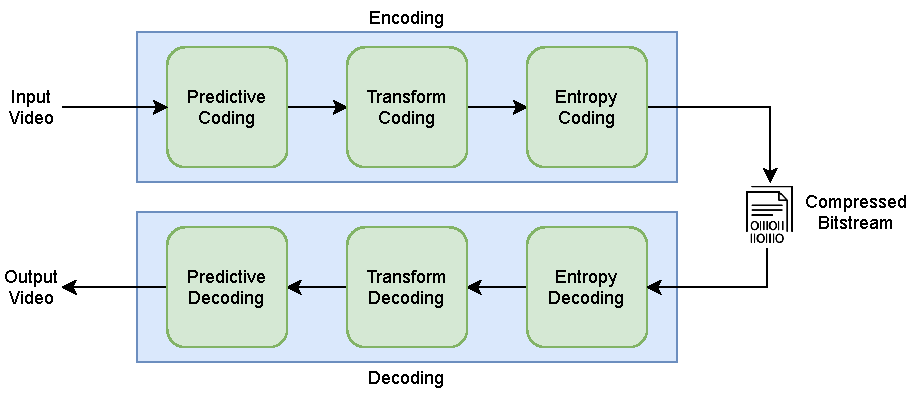
\includegraphics[width=0.8\linewidth]{img/comp_architecture.pdf}
  \caption[The typical video compression architecture]
  {
  The typical video compression architecture adapted from \cite{zhang_overview_2019}.
%   The encoder consists of predictive coding, transform coding, and entropy coding compresses the input video and generates the compressed bitstream. The decoder decompresses the bitstream in reverse order to the encoder and outputs the reconstructed video.
  }
  \label{fig:comp_architecture}
\end{figure}

There are two type of video coding; losssless coding and lossy coding. Lossless coding compresses the images and reconstructed images can be obtained after de-compression without any loss of information. Lossy coding however compresses the images by removing the less important information, which will sacrifice the image quality to the level the human visual system can be tolerant. Lossy compression is more widely used today since it allows much lower compressed size and more efficient than the lossless manner.

Since the first video compression standard of H.120 that has been developed in 1984, the various video compression standards have been developed such as MPEG and H.26X series \cite{zhang_overview_2019}.




The organization of Video Coding Expert Group (VCEG) of International Telecommunication Union (ITU-T) are developing H.26X series starting from the first standard of H.120, then developed H.261, H.262, H.263, H.264(AVC), and H.265 (HEVC). H.264 or so called Advanced Video Coding (AVC) were developed in 2003 and the typical architecture shown in Fig.\ref{fig:comp_architecture} were followed since H.264/AVC. H.264/AVC is the most widely used standard nowadays and supports up to 4k (4096×2304) resolution of video.


\section{Thesis preview}
\label{sec:introduction/thesis_preview}

As an organization of this thesis, we start by illustrating Chapter 1 the motivation for this research and providing history and background information for each object tracking and video compression concept. We will then explain the more detailed background information on the adopted methods in Chapter 2. Chapter 3 shows the methodologies and experimental procedures. Chapter 4 illustrates the results from the experiment and data analysis. Finally, we will conclude this research with the highlighted insights and future work in Chapter 5. The additional information is included in Appendix.
